%-------------------------------------------------------------------------------
% yum_menu_patch_sets
%-------------------------------------------------------------------------------
%
% \file        yum_menu_patch_sets.tex
% \library     Documents
% \author      Chris Ahlstrom
% \date        2016-02-27
% \update      2018-03-11
% \version     $Revision$
% \license     $XPC_GPL_LICENSE$
%
%     Provides the Menu / Instruments section of yoshimi-user-manual.tex,
%     for the 1.3.8 and above versions of Yoshimi.  That menu entry has changed
%     a lot.
%
%-------------------------------------------------------------------------------

\subsection{Menu / Patch Sets}
\label{subsubsec:menu_patch_sets}

   This new menu entry is part of the very nice reorganization and simplification
   of the handling of roots and banks in the new \textsl{Yoshimi}.  The
   \textbf{Patch Sets} menu replaces the old \textbf{Parameters} menu.  Do you
   like the new name?  The patch set saves all of the settings, including effects
   and instruments.  Patch sets will save all other instruments regardless of
   whether they are activated or not.  Default instruments are never saved, not
   even in patch sets, but if the parts are activated that fact \textsl{is}
   saved.  It is a part feature, not an instrument feature.

   \textsl{Yoshimi} stamps its configuration XML files with its own major and
   minor version numbers so it is possible to tell which version created the
   files, or whether they were created by \textsl{ZynAddSubFX}.

   The main dialog is somewhat similar in layout and function to the
   dialog shown in
   \figureref{fig:instruments_show_stored},
   for managing instruments in a selected bank.

\subsubsection{Menu / Patch Sets / Show Patch Banks...}
\label{subsubsec:menu_patch_sets_show_patch_banks}

   The \textbf{Banks} window has had some button shuffling, and one can
   import and export banks as well.

\begin{figure}[H]
   \centering
%  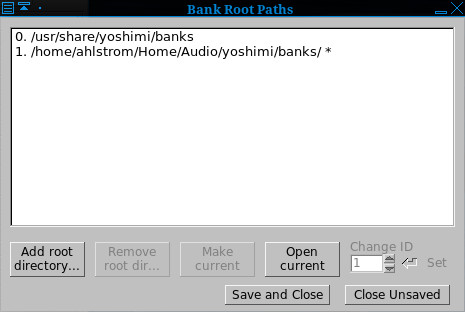
\includegraphics[scale=0.75]{menu/Instrument/show-banks-roots.jpg}
%  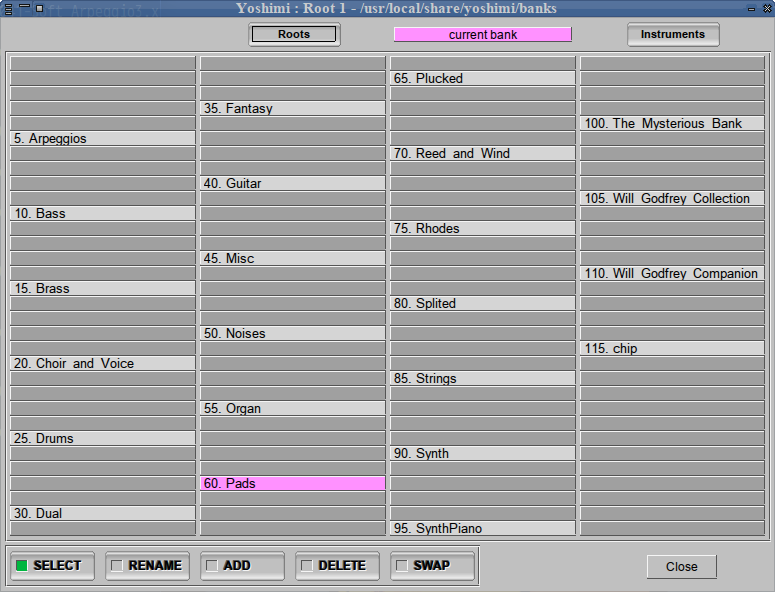
\includegraphics[scale=0.75]{1.3.9/patch_sets_show_patch_banks.png}
   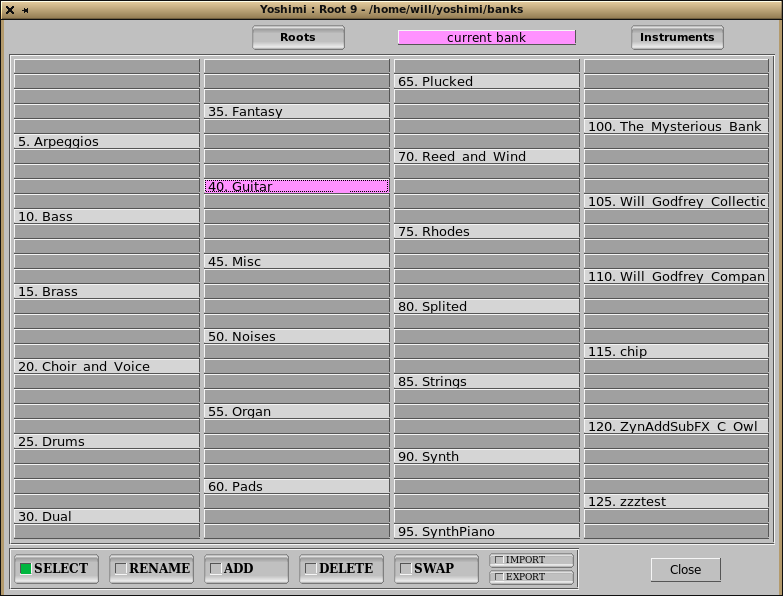
\includegraphics[scale=0.75]{1.5.7/Bank.png}
   \caption[Show Patch Banks]{Show Patch Banks}
   \label{fig:show_patch_banks}
\end{figure}

   Here is a list of the user-interface items in the patch-banks dialog:

   \begin{enumber}
      \item \textbf{Roots}
      \item \textbf{current bank}
      \item \textbf{Instruments}
      \item \textbf{Bank Matrix}
      \item \textbf{SELECT}
      \item \textbf{RENAME}
      \item \textbf{SAVE}
      \item \textbf{DELETE}
      \item \textbf{SWAP}
      \item \textbf{IMPORT}
      \item \textbf{EXPORT}
      \item \textbf{Close}
   \end{enumber}

   \setcounter{ItemCounter}{0}      % Reset the ItemCounter for this list.

   \itempar{Roots}{Roots!root directories}
   Show Patch Banks, Root Directories.
   To add a bank root path, delete a bank root path, or manage bank root path,
   press this button.  The result is somewhat similar to a file dialog,
   and is described in detail in
   \sectionref{subsubsec:menu_patch_sets_patch_bank_roots}, later in
   this sub-chapter.

   \itempar{current bank}{banks!current bank}
   This item is highlighted in pink, and the bank that is actually the current
   bank is also highlighted in pink.  There is no action associated with this
   user-interface element; it merely indicates the currently-selected bank.

   \itempar{Instrument}{banks!instrument}
   This button brings up an instruments window similar
   to the one shown in
   \figureref{fig:instruments_show_stored}, which shows
   the instruments collected in the currently-selected bank.
   Clicking on a bank in the dialog also brings up the instruments window.

   \itempar{Bank Matrix}{banks!matrix}
   This view shows all of the banks available in the current root.
   Left-clicking on a bank in the dialog brings up the Instruments window for
   that bank.
   Right-clicking on a bank in the dialog brings up the Instruments window for
   that bank, but also closes the banks window, to reduce clutter.

   \itempar{IMPORT}{banks!IMPORT}
   There are a number of benefits to using the IMPORT/EXPORT buttons
   rather than dealing with the directories externally.
   One has far greater control where things go when
   importing, and it's much easier to identify the bank to export.

   When importing or exporting,
   \textsl{Yoshimi} refuses to overwrite exisiting banks or
   directories. That is a flat refusal for exporting, but for importing it will
   add a numeric suffix to the name.

   Importing will copy in \textsl{only} files that
   \textsl{Yoshimi} understands, but will notify
   if there were other unrecognised types in there.
   Exporting just dumps out the entire bank contents.

   There are a number of banks in the wild that contain all sorts of extraneous
   stuff, usually copyright notices; one should use only the instrument
   text fields, provided for exactly that purpose.
   Oh, and one bank Will found had subdirectories with pictures,
   and they weren't small!

   In the main part \textbf{Instrument Edit} window there is a new
   \textbf{Default} button top right.
   See \sectionref{subsec:bottom_panel_instrument_edit}.

   We hope this encourages people
   to fill in the Author and Copyright information.
   To set it up, fill in the text field as normal,
   then, while holding down the Ctrl key, click on the button
   (left or middle mouse click) . This text will now be stored in
   one's
   \textsl{Yoshimi} configurionat directory,
   and whenever one creates a new instrument, just
   click on the \textbf{Default} button, and the saved text will be
   filled in.

   \itempar{EXPORT}{banks!EXPORT}
   Export of banks is described in the previous section.

   The buttons \textbf{SELECT}, \textbf{RENAME}, \textbf{SAVE},
   \textbf{DELETE}, and \textbf{SWAP} behave similarly to the same buttons in
   the Instruments window, as
   described in the discussion at
   \sectionref{subsubsec:menu_instrument_show}.

\subsubsection{Menu / Patch Sets / Load External...}
\label{subsubsec:menu_patch_sets_load}

   This menu entry simply brings up a file dialog, allowing the user to
   navigate to an arbitrary directory, and then to a solitary instrument file
   (\texttt{*.xmz}), and load it into the current set of parts.

\begin{figure}[H]
   \centering
   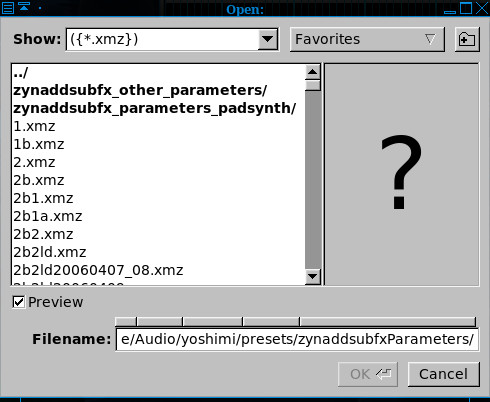
\includegraphics[scale=0.75]{menu/Parameters/open-parameters.jpg}
   \caption{Load Patch Set}
   \label{fig:yoshimi_menu_open_parameters}
\end{figure}

   These "xmz" files are normally found in a \texttt{presets} directory, but this
   operation allows access to banks that are not located in a particular root.

   When an "xmz" file is loaded, all of the instruments it contains are
   loaded sequentially into the Parts.  Thus, a number of instruments are loaded
   at once.  So, a patch set is a list of instruments that are related by
   being necessary for a given tune, rather than by being located in a
   particular bank.

%  In patch sets, \textsl{Yoshimi} will save named-but-disabled patches.
%  Currently, \textsl{ZynAddSubFX} does not, so be aware when transferring
%  data between the two synthesizers.

\subsubsection{Menu / Patch Sets / Save External...}
\label{subsubsec:menu_patch_sets_save}

   This menu entry simply brings up a file dialog, allowing the user to
   navigate to an arbitrary directory, and then save the current Part
   to a solitary instrument file (\texttt{*.xiz}).

   In patch sets, \textsl{Yoshimi} will save named-but-disabled patches.
   Currently, \textsl{ZynAddSubFX} does not, so be aware when transferring
   data between the two synthesizers.

\begin{figure}[H]
   \centering
   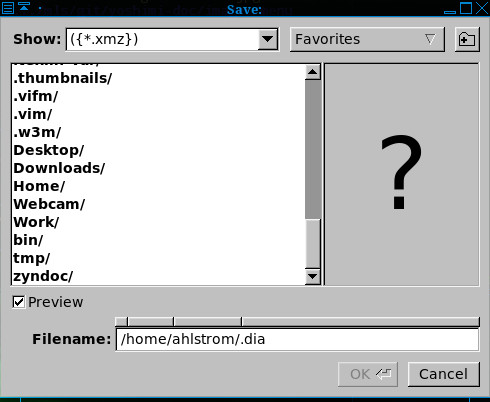
\includegraphics[scale=0.75]{menu/Parameters/save-parameters.jpg}
   \caption{Save Patch Set}
   \label{fig:yoshimi_menu_save_parameters}
\end{figure}

   Patch set saves include everything that is not part of the main
   configuration, and so saved patch sets
   includes \textbf{Master Volume} and \textbf{Detune}
   \textbf{Part} destinations, \textbf{Humanise},
   and more.
   If nothing has changed, then the following dialog is shown.

\begin{figure}[H]
   \centering
   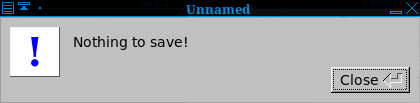
\includegraphics[scale=0.75]{menu/Parameters/nothing-to-save.jpg}
   \caption{Patch Set, Nothing to Save}
   \label{fig:yoshimi_menu_nothing_to_save_parameters}
\end{figure}

\subsubsection{Menu / Patch Sets / Recent Sets}
\label{subsubsec:menu_patch_sets_recent_sets}

   This menu entry brings up a dialog box with a list of the recent patch sets
   that have been loaded.  This item makes it easy to move around one's
   frequently-used banks.

\subsubsection{Menu / Patch Sets / Patch Bank Roots}
\label{subsubsec:menu_patch_sets_patch_bank_roots}

   \textsl{Yoshimi} (as installed by Debian Linux) provides a default bank at
   \texttt{/usr/share/yoshimi/banks}.
   To add one's own directory, click on the \textbf{Roots} button.
   It brings up the following dialog.

\begin{figure}[H]
   \centering
   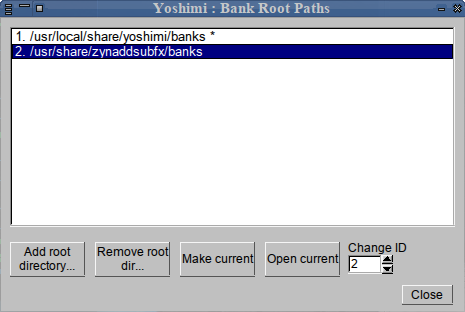
\includegraphics[scale=0.75]{1.3.9/patch_sets_bank_root_paths.png}
   \caption{Bank Root Paths}
   \label{fig:bank_root_paths}
\end{figure}

   This dialog has a number of buttons, some of which will be disabled if no
   directory in the list is selected.

   Then click on the "Add root directory..." button.  In the file dialog that
   appear, one can use the \textbf{Create Directory} button to make a new
   directory, if desired:

\begin{figure}[H]
   \centering
   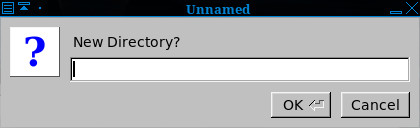
\includegraphics[scale=0.75]{menu/Instrument/new-directory.jpg}
   \caption{New Root Directory?}
   \label{fig:new_root_directory}
\end{figure}

   Otherwise, once can add an existing directory to the list.

   \setcounter{ItemCounter}{0}      % Reset the ItemCounter for this list.

   \itempar{Add root directory...}{Root Paths!add directory}
   Bank Root Paths, Add Root Directory.

   Once selected, one will see that
   \texttt{/usr/share/yoshimi/banks} or
   \texttt{/usr/local/share/yoshimi/banks}
   is marked with an asterisk.  One can select the new root directory via the
   file dialog that appears, and then make it the current root by clicking the
   \textbf{Make current} button.  Then the Banks dialog will show all the banks
   in that directory, one bank per subdirectory (each subdirectory "is" a
   bank).

   \itempar{Remove root directory...}{Root Paths!remove directory}
   Bank Root Paths, Remove Root Directory.
   If a path is selected, then this button is active, and can be used to
   delete the selected path from the "root paths" list. Note that this does
   \textbf{not} delete actual files, just removes the entry from the list.

   \itempar{Make current}{Root Paths!make current}
   Bank Root Paths, Make Current.
   \index{current!root}
   This button marks the currently-selected path as the "current root" path.

   \itempar{Open current}{Root Paths!open current}
   Bank Root Paths, Open Current.
   This button opens the current root path.
   (Does this work?)

   \itempar{Change ID}{Root Paths!change ID}
   Bank Root Paths, Change ID.
   This ID can be used to make the bank selectable via an extended MIDI
   control.

   Values: \texttt{0* to 127}

%-------------------------------------------------------------------------------
% vim: ts=3 sw=3 et ft=tex
%-------------------------------------------------------------------------------
